\chapter{Introduction}
\label{c.intro}

In the global and annual average, 65\% of rain falling on land returns to the atmosphere through evaporation [\cite{trenberth2007}].  Most of the evaporated water in vegetated regions first travels through plant tissue before evaporating, a process called transpiration [\cite{wilson2001comparison}, \cite{dirmeyer2005second}, \cite{jasechko2013terrestrial}].  Transpiration affects the atmosphere: a large transpiration flux can increase atmospheric moisture content and downstream precipitation [\cite{ISI:A1996VD58700003}] and can keep the land surface cool by consuming a large fraction of the net radiative energy at the land surface.  Plants actively control the rate of transpiration on short timescales by modulating the openness of small pores on their leaves called stomata.  Stomata respond to a range of environmental drivers, including water availability to roots and the drying capacity of the air, and different plant species respond differently to these drivers.  A forest composed of one tree species with certain stomatal responses can have different transpiration dynamics and thus affect the atmosphere differently than a forest composed of another tree species.  

In this dissertation, direct tree-level measurements of water use are analyzed to show that Douglas-firs (\textit{Pseudotsuga menziesii}, Figure \ref{fig:intro_treepics}(a)), a common evergreen needleleaf tree species in the Northern California Coast Range, decrease their transpiration sharply in the summer dry season in response to a dry root zone; and in contrast, broadleaf evergreen tree species, especially Pacific madrones (\textit{Arbutus menziesii}, Figure \ref{fig:intro_treepics}(b)), transpire maximally in the summer dry season because their transpiration is much less sensitive to a dry root zone and increases continually in response to increasing atmospheric evaporative demand.  These tree-level observations are scaled up to construct a bottom-up estimate of regional transpiration, and these regional estimates are used along with atmospheric models, one simple and one complex, to quantify the potential impact of species transpiration differences on regional summertime climate.  We extend the investigation of the sensitivity of California climate to evapotranspiration by testing the response of wind energy forecasts at a California wind farm to regional-scale perturbations in soil moisture, concluding that wind at this farm is sensitive on an operationally meaningful level to realistic soil moisture uncertainties.

\begin{figure}
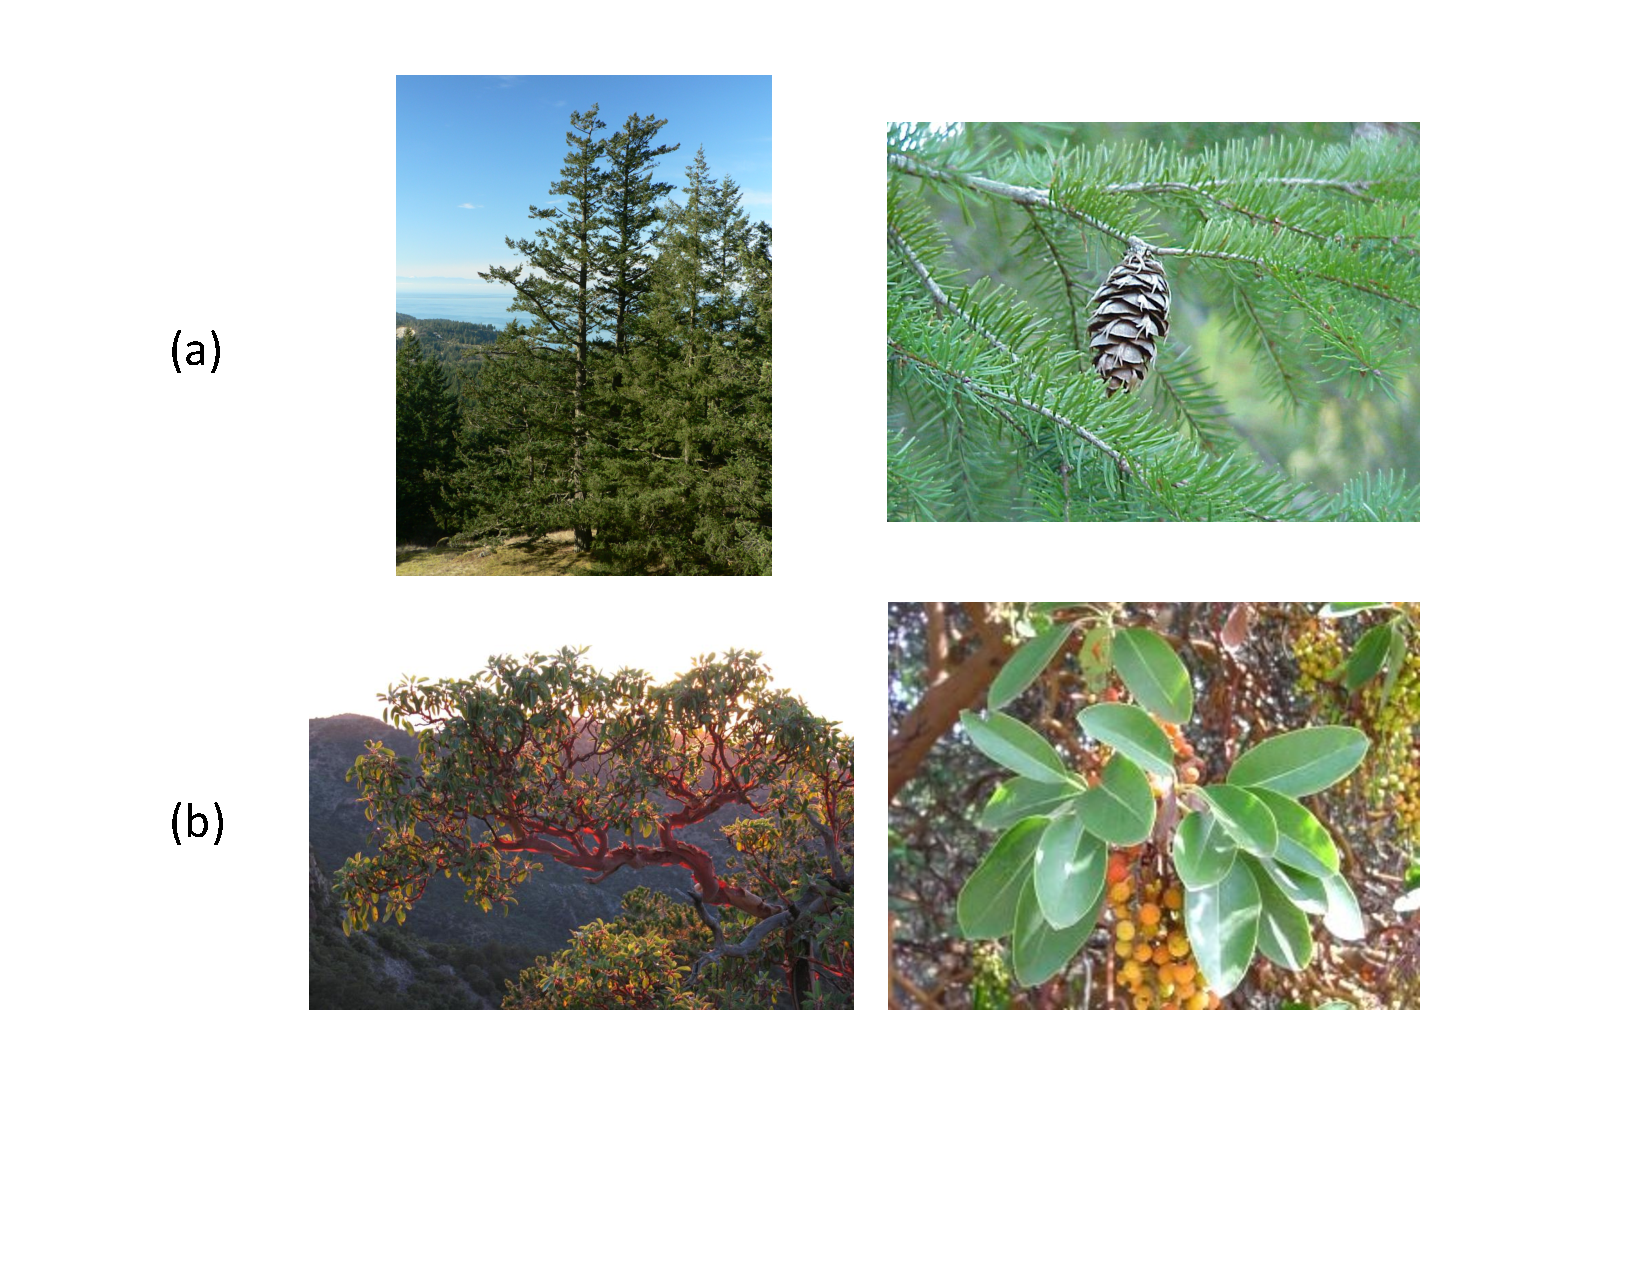
\includegraphics[width=0.9\textwidth]{ch0-introduction/tree_pics.pdf}
\caption{Photographs of (a) Douglas fir and (b) Pacific madrone trees.}
\label{fig:intro_treepics}
\end{figure}

\section{Background}

\subsection{Land surface energy balance}

The land surface gains energy by absorbing radiation from the sun (higher frequency radiation) and from the atmosphere (lower frequency radiation).  This energy gain is balanced by energy loss through emitted thermal radiation, conductive heat flux into the ground, and two types of turbulent heat fluxes.  These turbulent heat fluxes are (1) ``sensible heat'', or convective eddies carrying warmer air away from a hot land surface; and (2) ``latent heat'', which in atmospheric science refers to turbulent eddies carrying evaporated water vapor away from the land surface.  This evaporative flux is equivalent to an energy flux because the process of converting water from liquid to vapor consumes a large amount of energy; that energy is released later when the water vapor condenses, making the energy in water vapor ``latent''.

\begin{figure}
\begin{subfigure}{0.7\textwidth}
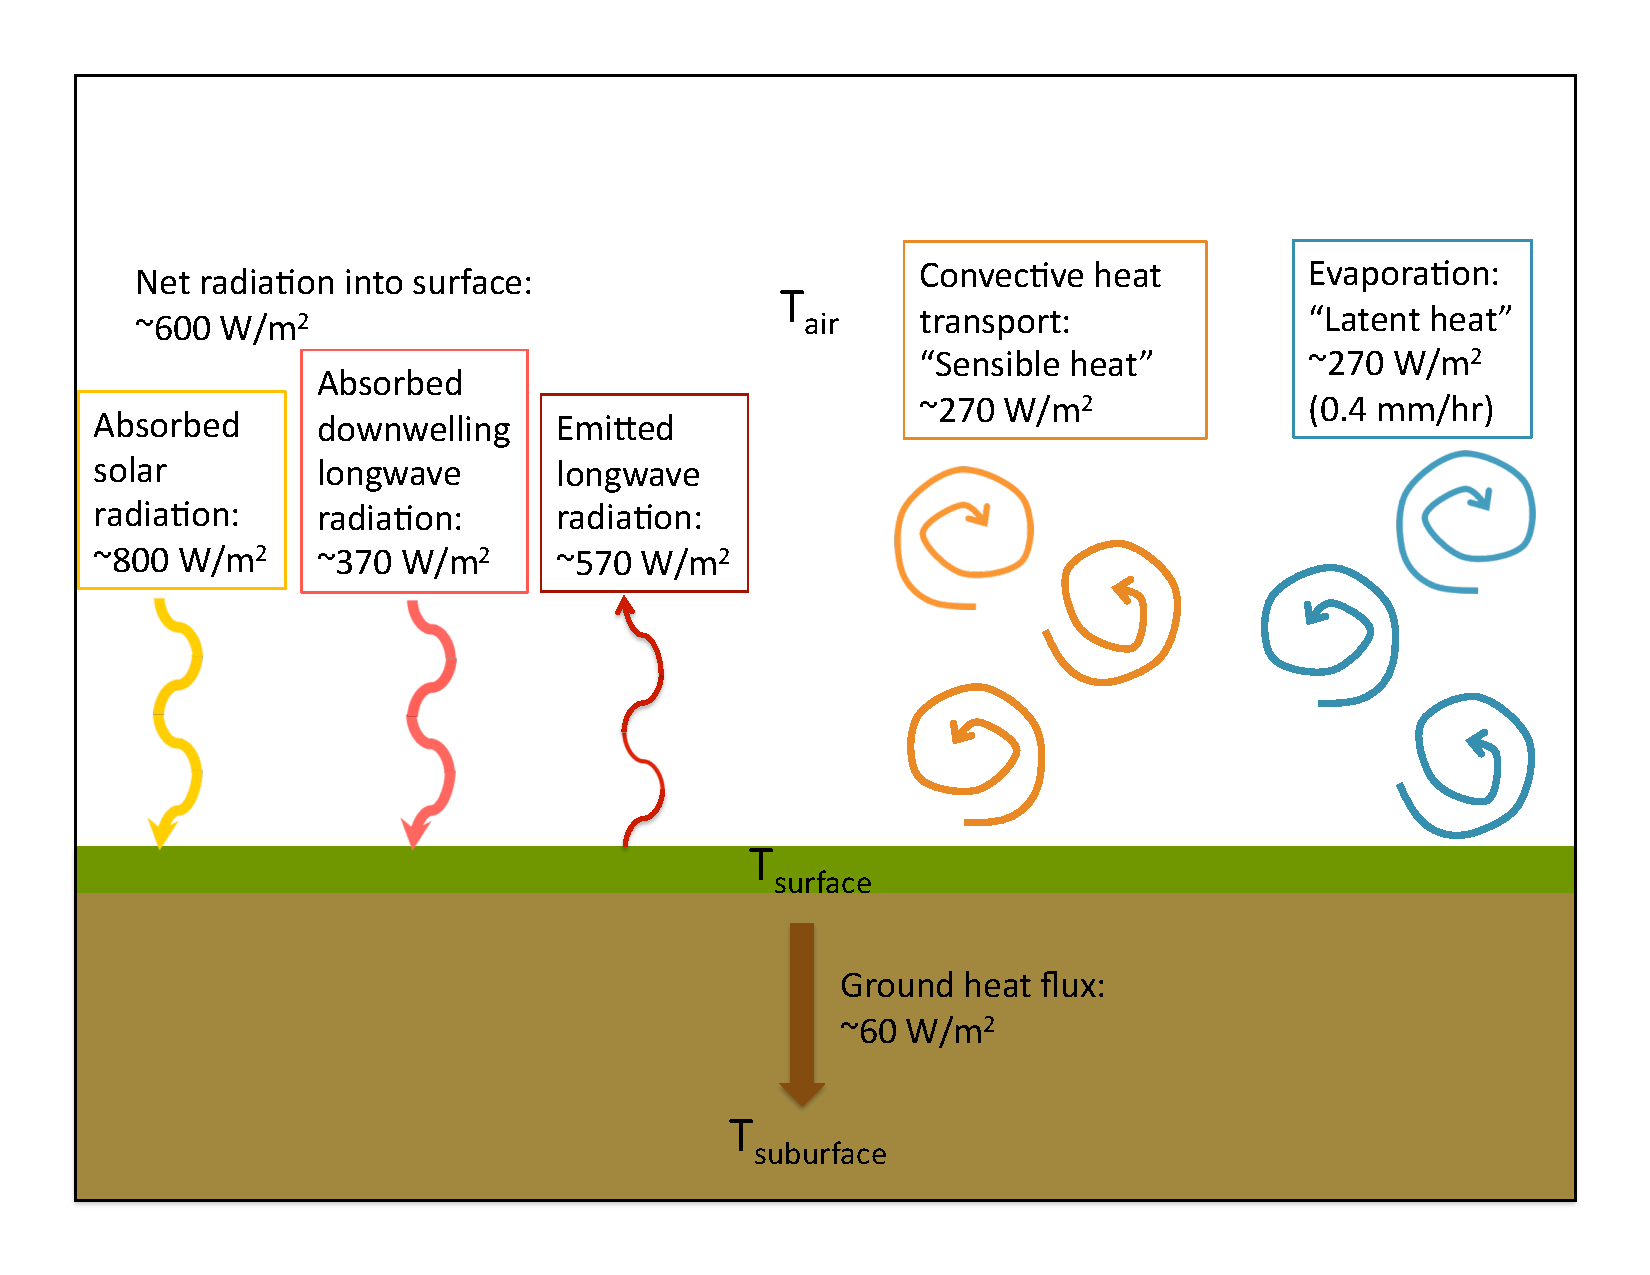
\includegraphics[width=\textwidth]{ch0-introduction/energy_balance_wet.pdf}
\caption{}
\end{subfigure}
\begin{subfigure}{0.7\textwidth}
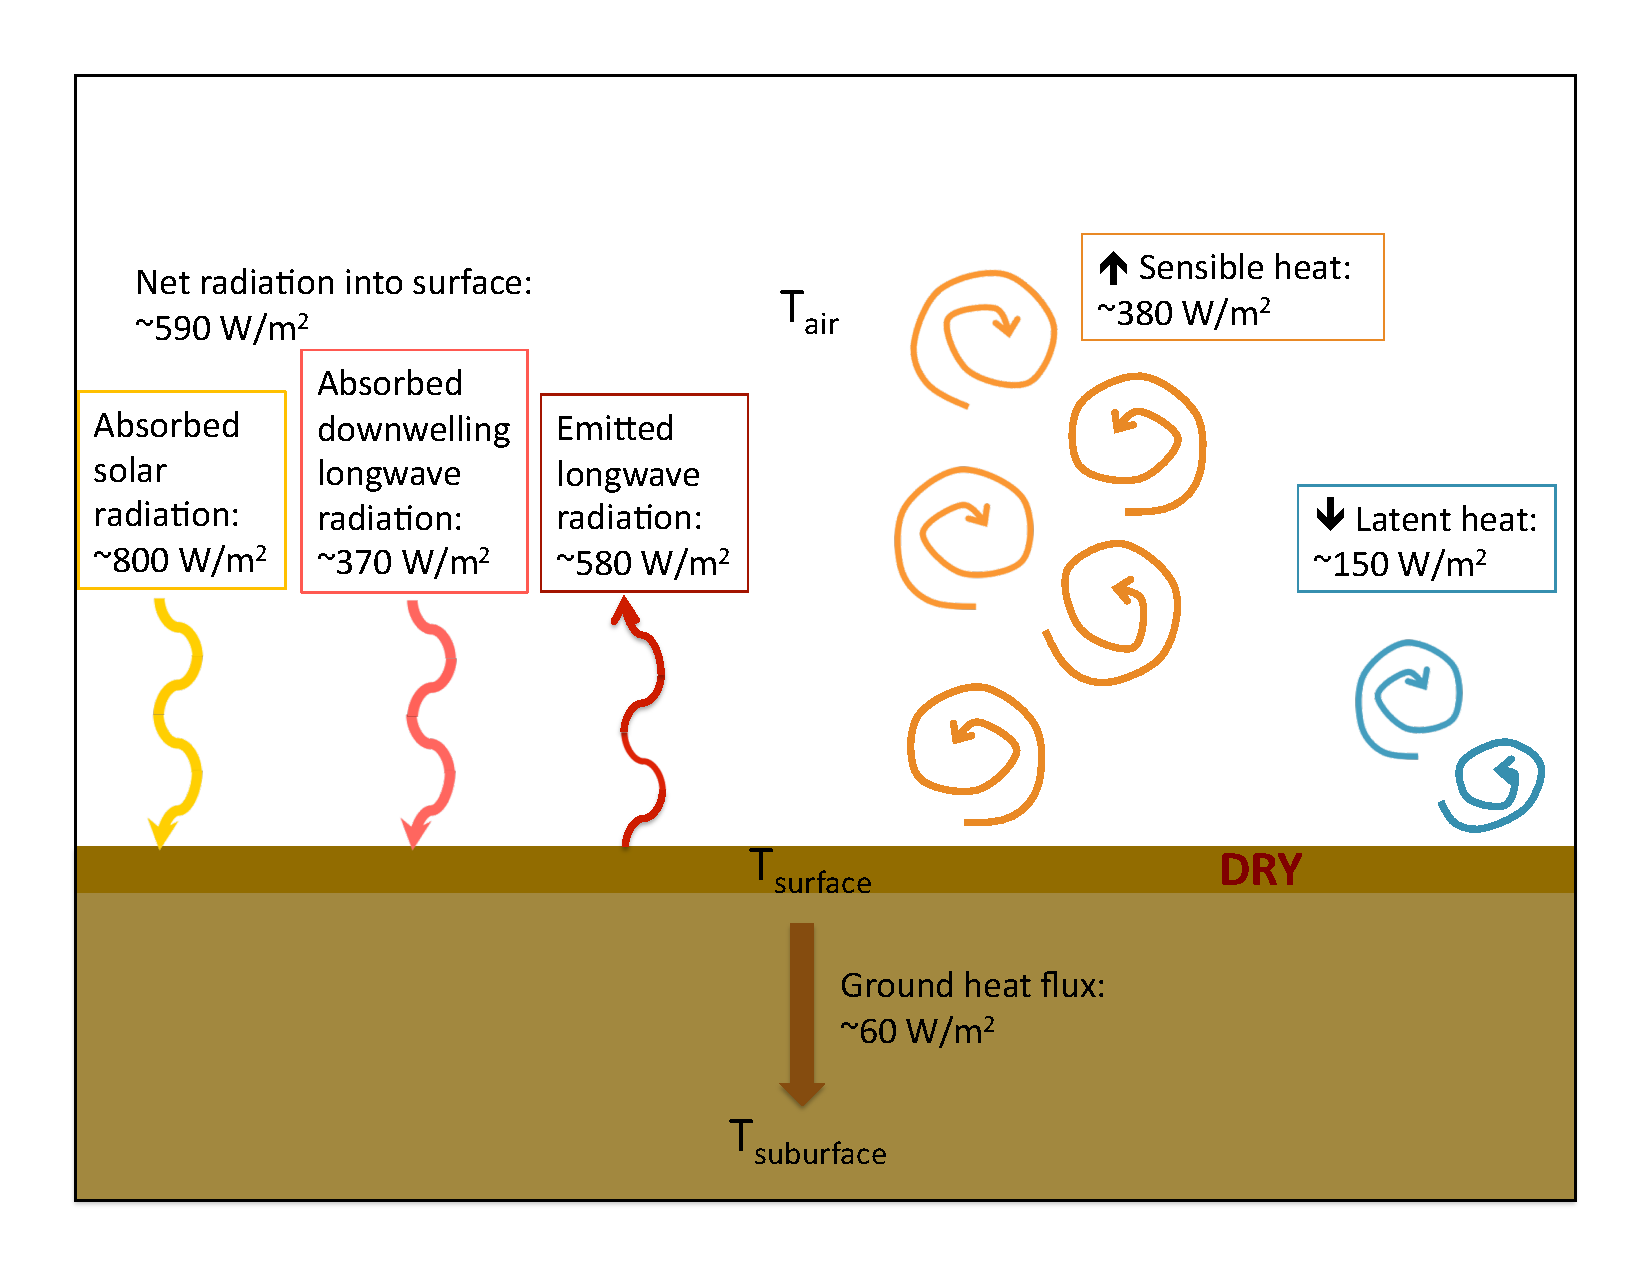
\includegraphics[width=\textwidth]{ch0-introduction/energy_balance_dry.pdf}
\caption{}
\end{subfigure}
\caption{Typical midlatitude midday land surface energy balance for (a) wet soil and (b) dry soil.  Net radiation is slightly lower in the dry case because the higher surface temperature leads to greater emitted longwave radiation.  Flux values from e.g. \cite{bonan}, \cite{teuling2010contrasting}.}
\label{fig:intro_enbal}
\end{figure}

Figure \ref{fig:intro_enbal} shows the terms of the midday land surface energy balance when the soil is wet (Figure \ref{fig:intro_enbal}(a)) and when the soil is dry (Figure \ref{fig:intro_enbal}(b)).  In the midlatitudes at midday, typical net radiation is approximately 600 W/m$^2$, and roughly 5-10\% of that energy goes to the ground heat flux.  When water is readily available at the surface, the latent heat flux can consume 50\% or more of the net radiation minus ground heat flux.  A large amount of energy is required to evaporate water (evaporating a depth of 1 mm of water requires 2.26\e{^6} J/m$^2$), so even the relatively high latent heat flux of 270 W/m$^2$ translates to only 0.4 mm liquid water evaporated per hour.  Water limitation at the land surface (for instance, because of dry surface soil in a bare ground case, or because of closed stomata in a vegetated setting; Figure \ref{fig:intro_enbal}(b)) reduces the latent heat flux and thus increases the surface temperature and the sensible heat flux to the lower atmosphere.

\subsection{Influence of evapotranspiration on the atmosphere}

The partitioning of surface energy between latent heat and sensible heat affects atmospheric temperature, humidity, and circulations.  During the daytime, sensible heat drives buoyant convection from the surface, deepening the well-mixed atmospheric boundary layer (the lower 1-2 km of the daytime atmosphere that interacts rapidly with the surface).  Greater evapotranspiration reduces the land surface temperature and the sensible heat flux.  With a larger flux of water vapor and a smaller flux of sensible heat, the atmospheric boundary layer tends to be shallower, cooler, and moister, with the exact outcome depending on background conditions like radiation, clouds, and free troposphere stability and humidity [\cite{bonan}, \cite{garratt1994atmospheric}].

Horizontal differences in the partitioning of turbulent heat fluxes can drive local- to regional-scale circulations.  In areas with more sensible heat flux, the boundary layer tends to warm, reducing the density of the air and generating a zone of low pressure.  The difference in pressure relative to adjacent regions with lower sensible heat flux (and thus cooler temperature, higher low-level density and higher pressure) can drive wind circulations.  Coherent circulations can form when the length scale of land surface heat flux variation is 5-10 km or greater [\cite{avissar1998evaluation}].

\subsection{Plant control of transpiration}

Transpiration occurs because plants must open their stomata (approximately 10 $\mu$m-scale pores on the surface of leaves) in order to take in carbon dioxide for photosynthesis, and in the process, water from the wet interior of the leaf evaporates and exits the stomata [\cite{bonan}].  Thus plants (especially those with the C3 carbon fixation pathway, in which CO$_2$ is drawn directly from air in the stomatal cavity during photosynthesis) must continually balance the gain of carbon dioxide against the loss of water, particularly in water-limited ecosystems.  Plants actively control the openness of their stomata in order to optimize this balance.  The rate of water loss ($E$, L/s) depends on the stomatal conductivity ($g_s$, a measure of openness, L/s/kPa) and on the difference in vapor pressure between the interior of the leaf and the outside air (measured by vapor pressure deficit, or $VPD$, kPa):

\begin{equation}
E = g_s * VPD ,
\end{equation}
where
\begin{equation}
VPD = e_{sat}(T_{air}) - e_{air}
\end{equation}
and $e_{sat}(T_{air})$ is the saturation vapor pressure at air temperature (kPa) and $e_{air}$ is actual vapor pressure of the air (kPa).

The stomatal conductivity responds on short timescales (seconds to minutes) to environmental conditions, including light, $VPD$, carbon dioxide concentration, and root-zone moisture availability.

Different plant species employ different strategies to balance carbon gain against water loss.  Rapid or excessive water loss can damage plant tissue by causing xylem cavitation, or gas intrusion into the plant's hydraulic system.  However, extended periods of closed stomata can deplete a plant's sugar reserves if the rate of metabolizing those sugars (respiration) exceeds the rate of photosynthesis.  Some plants adopt a hydraulically cautious strategy, closing stomata quickly as atmospheric evaporative demand grows and as root-zone water is depleted, with the advantage of maintaining a larger ``hydraulic safety margin,'' or difference between actual xylem water potential and the xylem water potential at which cavitation occurs [\cite{choat2012global}]. One significant downside of this strategy, of course, is the reduced opportunity to take in carbon dioxide for photosynthesis.  At the other end of the spectrum, some species adopt a hydraulically riskier strategy, keeping their stomata more open even as atmospheric evaporative demand increases and the root-zone dries.  With this strategy, plants can fix more carbon dioxide but maintain a lower hydraulic safety margin during times of water stress.

In periods of moderate water stress such as the California summer dry season, the hydraulically cautious strategy translates to lower transpiration than the hydraulically risky strategy, as the cautious species close their stomata more quickly in response to limited water availability and high atmospheric evaporative demand.  Among the species studied in this dissertation, as in \cite{choat2012global}, the hydraulically cautious species is a gymnosperm and the hydraulically riskier species are angiosperms.  However, differences among the angiosperms were also apparent; in particular, one angiosperm broadleaf evergreen tree species, Pacific madrone, was markedly less sensitive to root-zone water limitation than the other angiosperm broadleaf evergreen species.  These differences are estimated to be strong enough to influence regional-scale atmospheric boundary layer temperature, depth, and humidity.  These results suggest that species-specific understanding of stomatal response will give greater accuracy in evapotranspiration estimates, but this must be balanced against the difficulty of quantifying many more vegetation subgroups' stomatal response parameters.

\section{Scientific contributions}

In Chapter \ref{c.sapflow}, the seasonality of evergreen tree transpiration in a Mediterranean climate is investigated, using direct observations of tree water use. Mediterranean climates pose particular challenges for trees because the season of water availability (winter) is out of phase with the season of light availability and atmospheric moisture demand (summer). The analysis of sap flow measurements shows that two common evergreen tree species in Northern California have different seasons of peak transpiration.  Douglas-firs (\textit{Pseudotsuga menziesii}) maintain significant transpiration through the winter rainy season and transpire maximally in the spring, followed by a sharp decline in transpiration in the summer dry season.  Pacific madrones (\textit{Arbutus menziesii}), and to a lesser extent other broadleaf evergreen species (\textit{Quercus wislizeni}, \textit{Notholithocarpus densiflorus}, \textit{Umbellularia californica}), in contrast, transpire maximally in the summer dry season. The difference in transpiration seasonality arises from different sensitivities to atmospheric evaporative demand and root-zone moisture, and the difference is large enough that regional-scale species shifts between evergreen tree species could cause marked changes in regional evapotranspiration.

In Chapter \ref{c.BL}, we estimate the effect of these tree species differences in water use on the atmospheric boundary layer, using two atmospheric models, one simple and one comprehensive. We compare scenarios of regional-scale forest conversion from 100\% Douglas fir (\textit{Pseudotsuga menziesii}) to 100\% Pacific madrone (\textit{Arbutus menziesii}), the two species with the most different water use strategies.  In both models, when soils are dry, the summertime afternoon mixed layer over the Pacific madrone forest is cooler (by ~1-1.5 deg C), moister (by ~1 g/kg), and shallower (by ~200-500 m) than that over the Douglas fir forest.  The near-surface temperature and humidity differences between the species cases, as simulated in a regional atmospheric model (the Weather Research and Forecasting model, or WRF), are even larger: over the madrone forest, the air at 2 m above ground is ~1.5-2.5 deg C cooler and ~2-3 g/kg moister than the air at 2 m above ground over the douglas fir forest.  These results suggest that shifts in species composition of Northern California forests could affect the atmospheric boundary layer in the dry season, and these potential effects should be considered in forest management decisions and assessment of regional climate change impacts.

Soil moisture, through its influence on the land surface energy balance, affects not only temperature and humidity but also regional-scale atmospheric circulations.  In Chapter \ref{c.wind}, the effect of model soil moisture on the accuracy of wind energy forecasts is quantified for a Northern California wind farm, using the WRF model.  Winds at this site, the Solano Wind Project, are most sensitive to soil moisture changes in the Central Valley region.  When Central Valley soils are very dry, afternoon Solano wind is up to 2.5 m/s faster (1 m/s faster on average) than when Central Valley soils are moderately moist.  The wind speed changes are concentrated in the afternoon (10:00 to 18:00 local time) at Solano, causing the afternoon wind speed ramp-up to shift.  Decreases in low-level (< 300 m) pressure in the Central Valley relative to the Central Coast, caused by increased land surface heating over drier soil, drive wind speed increases at Solano.  Errors in weather-model-derived soil moisture of 0.1-0.15 m$^3$/m$^3$, documented in previous analyses [\cite{marshall2003impact}, \cite{godfrey2008soil}], are large enough to alter Solano wind speed forecasts by 1-3 m/s, which can translate to differences in forecasted wind energy of 15-40\% of a wind farm's maximum rated power.

\section{Methodological contributions}

This thesis contributes methodological innovations to the study of forest transpiration and the study of evapotranspiration effects on regional climate.  These innovations include new applications of statistical techniques to a high-frequency and long-term sap flow dataset, scaling of sap flow measurements to regional transpiration estimates using a publicly-available forest inventory dataset, comparing this sap-flow-derived regional transpiration estimate with satellite-based estimates, using atmospheric models of varying complexity to quantify the atmospheric response to species differences in transpiration, and using an atmospheric model to systematically test the effect of soil moisture uncertainty on wind energy predictions.

This diversity of methods is needed because of the difficulty of relating measurements of evapotranspiration at local and regional scales.  Techniques such as leaf chambers and sap flow instrumentation can measure transpiration at the individual leaf- or tree-level; however, they are labor-intensive and difficult to deploy beyond the scale of a single plot of land.  Evapotranspiration can be estimated at the 1-10 km$^2$ scale with eddy covariance techniques or at the 1-km$^2$-to-continental scale with satellite observation-model hybrids.  Each of these methods has associated uncertainties, and moreover, they estimate the aggregated evapotranspiration, meaning that observed dynamics cannot directly be attributed to any one species or subgroup of plants.  In Chapter \ref{c.sapflow}, we link individual tree-level observations with the regional  scale by using principal component analysis (PCA) and Markov chain Monte Carlo (MCMC) parameter estimation to quantify dominant and consistent patterns that might hold at larger scales.  We build a bottom-up estimate of regional transpiration using these dominant patterns together with a regional inventory of tree sizes and abundances.  This bottom-up inventory suggests that satellite-based, top-down estimates overestimate dry season transpiration in the Northern California Coast Range, possibly because they do not reduce estimated transpiration enough in response to dry soils.

Another methodological contribution of this dissertation is the integration of sap flow measurements with atmospheric models to estimate the atmospheric boundary layer response to species differences in transpiration.  In Chapter \ref{c.BL}, we use two atmospheric models of very different degrees of complexity to independently confirm the effects on the atmospheric boundary layer.  The first model, a simple one-dimensional slab model of the atmospheric boundary layer, represents boundary layer growth by convective entrainment of free tropospheric air; it neglects complicating processes such as clouds, terrain, and advection and any other lateral heterogeneity, and its representation of convective turbulence is very simplistic.  The second model, a three-dimensional regional atmospheric model, represents many more processes (e.g. radiation, clouds, turbulence) and allows for lateral variation and advection.  Testing the atmospheric boundary layer response to species difference in transpiration using these two levels of model complexity lends credence to the results.

Chapter \ref{c.wind} of this dissertation applies the modeling of evapotranspiration-atmosphere interactions to a new use: wind energy forecasting.  We show that soil moisture errors of a magnitude known to exist in reanalysis datasets can influence wind energy forecasts at one California wind farm in an operationally significant way.  The study's systematic perturbation of soil moisture in an atmospheric model, and its mechanistic analysis of wind response, establish a prototype for similar studies at other wind farms.  Such studies could support measurement campaigns and data assimilation to improve wind energy forecast accuracy.

\section{Further questions}

This work raises new questions about the effects of species differences in water use strategies on watersheds and the atmosphere.  First, where do Douglas firs and Pacific madrones (two species with very different water use patterns) access subsurface water, and do they tap into distinct water stores?  There is some evidence that Pacific madrones, which transpire maximally in the summer dry season, may have access to both deeper water, via deeper roots than Douglas firs, and more tightly bound water, by reaching lower tissue water potentials (Chapter \ref{c.sapflow} Discussion).  Understanding species differences in subsurface water access is essential for a mechanistic understanding of water movement through the subsurface-vegetation-atmosphere system.  Such a mechanistic understanding will enable informed projections of the effect of changes in species abundance on streamflow (to what extent does each species tap into reservoirs that contribute to summertime baseflow?) and the resilience of each species to longer and more intense future droughts (what will happen to each species's water store in such droughts?  Is deeper water more protected from depletion during drought, and does it thus confer resilience on deep-rooted species?)

The different hydraulic strategies outlined here also raise questions about these tree species's resilience or mortality in response to drought.  The causes of tree mortality, and the relative importance of carbon starvation vs. hydraulic failure, are still debated [\cite{sala2010physiological}].  Future work should investigate how the different hydraulic strategies employed by Douglas firs and Pacific madrones make them more or less susceptible to drought-induced mortality.  How will the species distribution in the Northern California Coast Range respond to a warmer climate (will there be more droughts? Will they be longer or more intense or both?  How does each species respond to an unusually long drought?  To an unusually intense drought?)

A major challenge in evapotranspiration research is heterogeneity and scaling up from local-scale measurements.  In this thesis, very local measurements of tree water use are generalized across aspects, slopes, geologies, and elevations.  More work is needed in the evergreen forests of the Northern California Coast Range to sample tree water use in a wider range of these conditions, and among other common tree species not sampled here.  Such observations are necessary in order for generalizable patterns to emerge from the specificity and heterogeneity of each individual field site.
